%!TEX root = /Users/louis/Documents/PhD/Deliverables/Thesis/thesis.tex

\section{MDE Tools}
\label{sec:mde_tools}
For MDE to be applicable in the large, and to complex systems, mature and powerful tools and languages must be available. Such tools and languages are beginning to emerge  This section discusses two MDE tools that are well-suited for MDE research and are used in the remainder of the thesis.

Section~\ref{subsec:emf} provides an overview of the Eclipse Modelling Framework (EMF) \cite{emf}, which implements MOF and underpins many contemporary MDE tools and languages, facilitating their interoperability. Section~\ref{subsec:epsilon} discusses Epsilon \cite{epsilon}, an extensible platform for the specification of model management languages. The highly extensible nature of Epsilon (which is described below) makes it an ideal host for the rapid prototyping of languages and exploring research hypotheses.  

The purpose of this section is to review EMF and Epsilon, which are used throughout the remainder of the thesis, and not to provide a thorough review of all MDE tools. There are many other MDE tools and environments that this section does not discuss, such as ATL \cite{atl} and VIATRA \cite{viatra} for M2M transformation, oAW \cite{oaw} for model transformation and validation, and MOFScript \cite{oldevik05toward} and XPand \cite{xpand} for M2T transformation.

\subsection{Eclipse Modelling Framework (EMF)}
\label{subsec:emf}
\cite{eclipse} is an open-source community seeking to build an extensible development platform. The Eclipse Modelling Framework (EMF) project \cite{emf} enables MDE within Eclipse. EMF provides a modelling framework with code generation facilities, and a meta-modelling language, Ecore, that implements the MOF 2.0 specification \cite{mof}. EMF is arguably the most widely-used contemporary MDE modelling framework.

EMF is used to generate metamodel-specific editors for loading, storing and constructing models. EMF model editors comprise a navigation view for specifying the elements of the model, and a properties view for specifying the features of model elements. Figure~\ref{fig:emf_model_editor} shows an EMF model editor for a simplistic state machine language. The navigation (or tree) view is shown in the top pane, while the properties view is shown in the bottom pane.

\begin{figure}[htbp]
  \begin{center}
    \leavevmode
    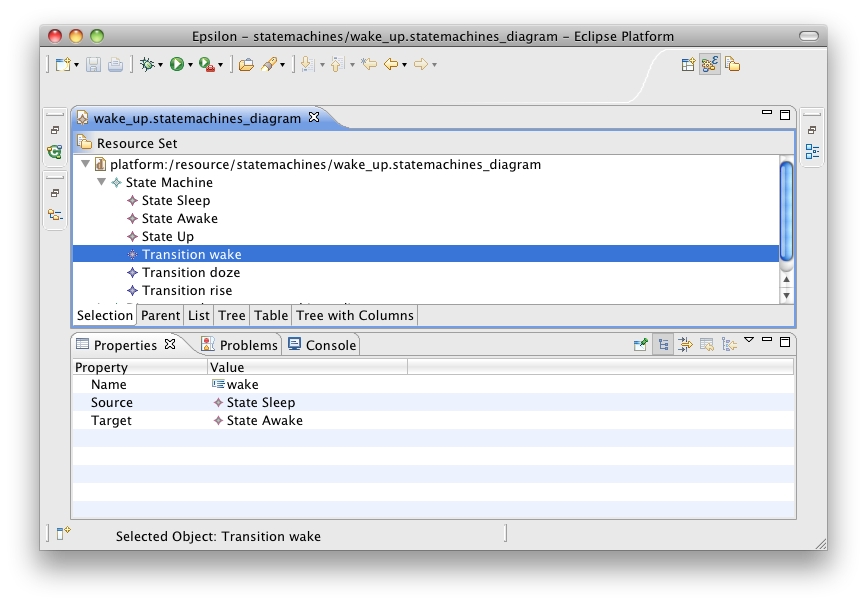
\includegraphics[width=10cm]{2.Background/images/emf_model_editor.png}
  \end{center}
  \caption{EMF state machine model editor.}
  \label{fig:emf_model_editor}
\end{figure}

Users of EMF can define their own metamodels in Ecore, the metamodelling language and MOF implementation of EMF. EMF provides two metamodel editors, tree-based and graphical. Figure~\ref{fig:emf_metamodel_editor_tree} shows the metamodel of a simplistic state machine language in the tree-based metamodel editor. Figure~\ref{fig:emf_metamodel_editor_diagrammatic} shows the same metamodel in the graphical metamodel editor. Like MOF, the graphical metamodel editor uses concrete syntax similar to that of UML class diagrams. Emfatic \cite{emfatic} provides a further, textual metamodel editor for EMF, and is shown in Figure~\ref{fig:emf_metamodel_editor_textual}. The editors shown in Figure~\ref{fig:emf_metamodel_editor_tree}, \ref{fig:emf_metamodel_editor_diagrammatic} and \ref{fig:emf_metamodel_editor_textual} are being used to manipulate the same underlying metamodel, but using different syntaxes. A change to the metamodel in one editor can be propagated automatically to the other two.

\begin{figure}[htbp]
  \begin{center}
    \leavevmode
    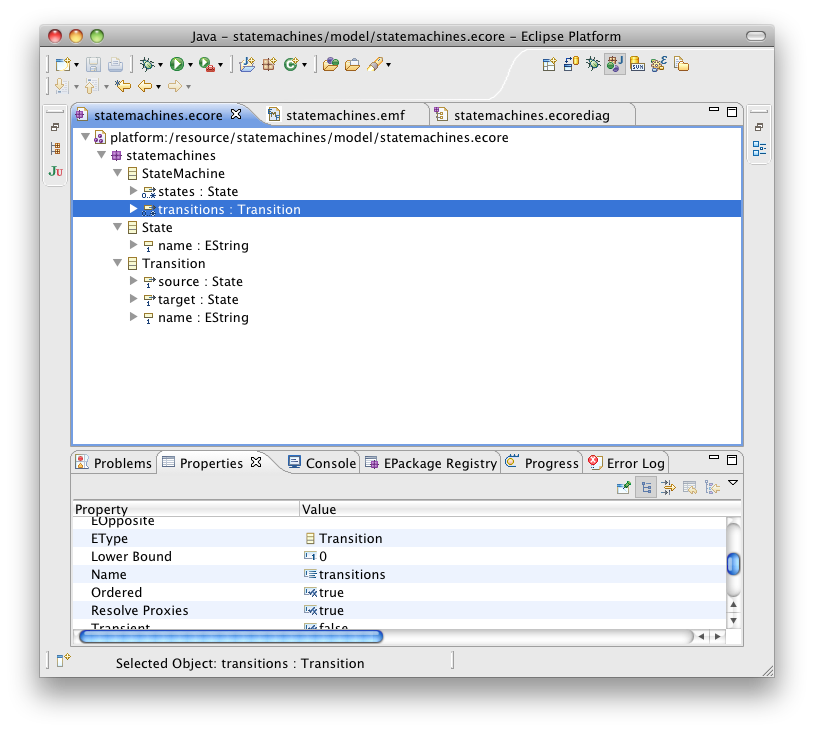
\includegraphics[width=10cm]{2.Background/images/emf_metamodel_tree.png}
  \end{center}
  \caption{EMF's tree-based metamodel editor.}
  \label{fig:emf_metamodel_editor_tree}
\end{figure}

\begin{figure}[htbp]
  \begin{center}
    \leavevmode
    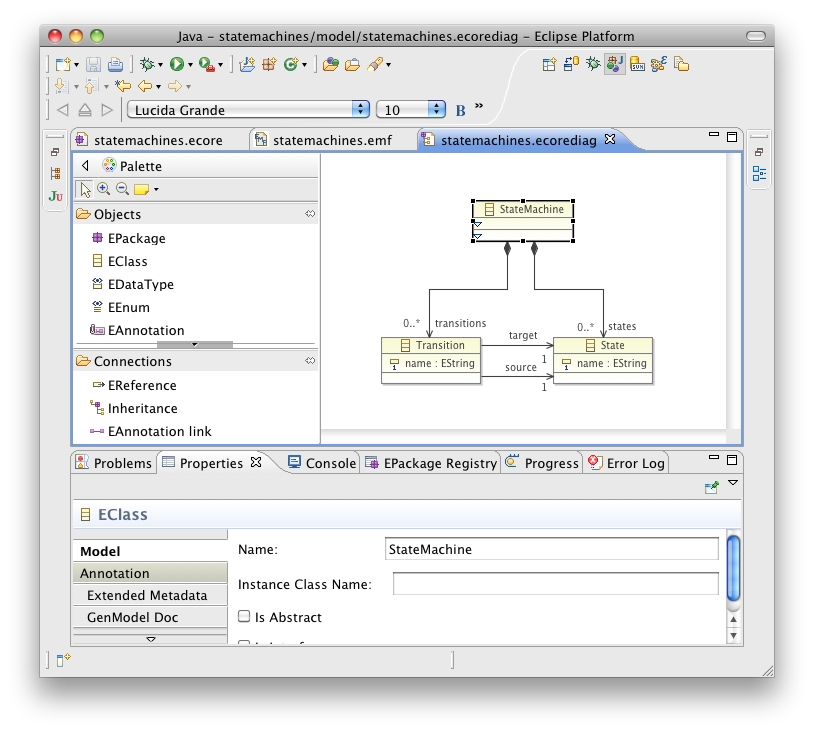
\includegraphics[width=10cm]{2.Background/images/emf_metamodel_diagrammatic.png}
  \end{center}
  \caption{EMF's graphical metamodel editor.}
  \label{fig:emf_metamodel_editor_diagrammatic}
\end{figure}

\begin{figure}[htbp]
  \begin{center}
    \leavevmode
    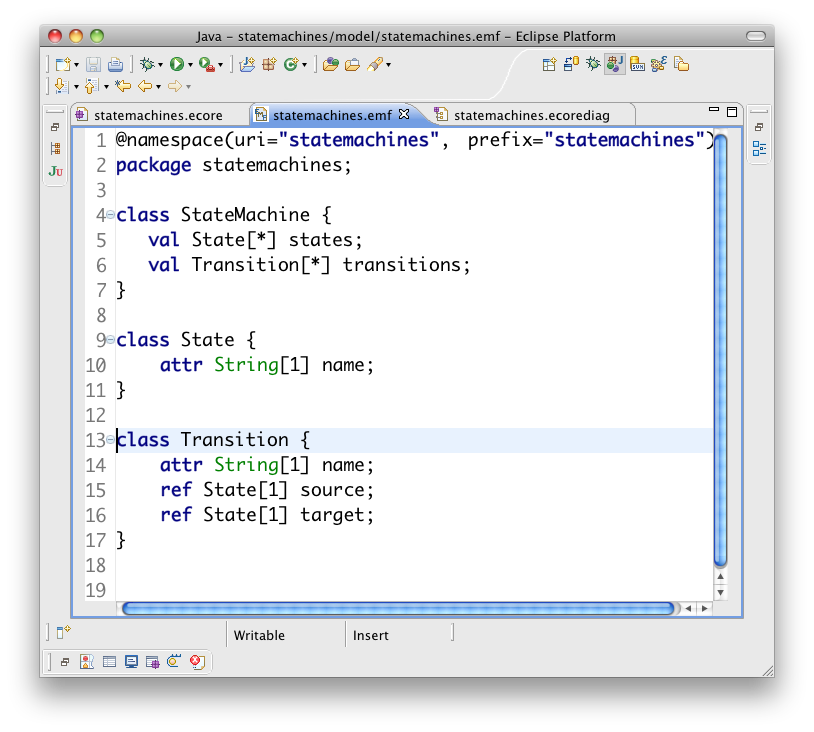
\includegraphics[width=10cm]{2.Background/images/emf_metamodel_textual.png}
  \end{center}
  \caption{The Emfatic textual metamodel editor for EMF.}
  \label{fig:emf_metamodel_editor_textual}
\end{figure}

From a metamodel, EMF can generate an editor for models that conform to that metamodel. For example, the simplistic state machine metamodel specified in Figures~\ref{fig:emf_metamodel_editor_tree}, \ref{fig:emf_metamodel_editor_diagrammatic} and \ref{fig:emf_metamodel_editor_textual} was used to generate the code for the model editor being used in Figure~\ref{fig:emf_model_editor}. The model editors generated by EMF include mechanisms for persisting models to and from disk. As prescribed by MOF, EMF typically generates code that persists models using XMI \cite{xmi}, a dialect of XML optimised for model interchange.

The Graphical Modeling Framework (GMF) \cite{gronback09emp} is used to specify generate graphical model editors from metamodels defined with EMF. Figure~\ref{fig:gmf_model_editor} shows a model editor produced with GMF for the simplistic state machine language described above. GMF itself uses a model-driven approach: users specify several models, which are combined, transformed and then used to generate code for the resulting graphical editor. 

\begin{figure}[htbp]
  \begin{center}
    \leavevmode
    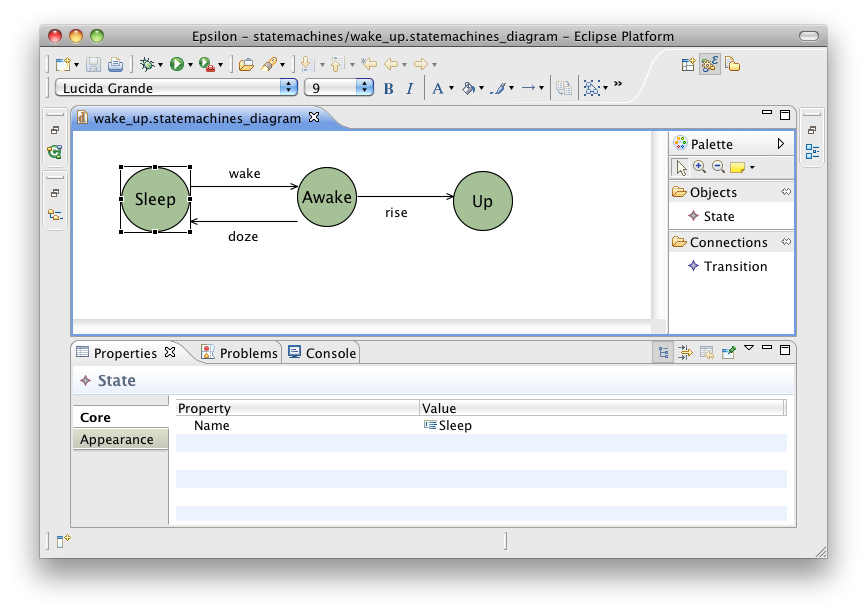
\includegraphics[width=10cm]{2.Background/images/gmf_model_editor.png}
  \end{center}
  \caption{GMF state machine model editor.}
  \label{fig:gmf_model_editor}
\end{figure}

Many MDE tools are interoperable with EMF, enriching its functionality. The remainder of this section discusses one tool that is interoperable with EMF, Epsilon, which is a suitable platform for rapid prototyping of model management languages and, hence, is useful for performing MDE research.

\subsection{Epsilon}
\label{subsec:epsilon}
The Extensible Platform for Specification of Integrated Languages for mOdel maNagement (Epsilon) \cite{epsilon} is a suite of tools and domain-specific languages for MDE. Epsilon comprises several integrated model management languages -- built atop a common infrastructure -- for performing tasks such as model merging, model transformation and inter-model consistency checking \cite{kolovos09thesis}. Figure \ref{fig:epsilon} illustrates the various components of Epsilon.

Whilst many model management languages are bound to a particular subset of modelling technologies, limiting their applicability, Epsilon is metamodel-agnostic: models written in any modelling language can be manipulated by Epsilon's model management languages \cite{kolovos06eol}. Currently, Epsilon supports models implemented using EMF, MOF 1.4, XML, or Community Z Tools (CZT)\footnote{\url{http://czt.sourceforge.net/}}. Interoperability with further modelling technologies can be achieved by extension of the Epsilon Model Connectivity (EMC) layer. 

\begin{figure}[htbp]
  \begin{center}
    \leavevmode
    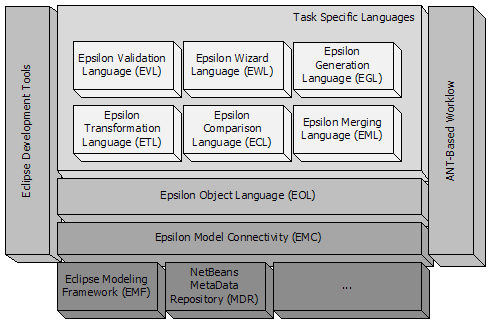
\includegraphics[scale=0.6]{2.Background/images/epsilon.png}
  \end{center}
  \caption{The architecture of Epsilon, taken from \cite{rose08egl}.}
  \label{fig:epsilon}
\end{figure}

The architecture of Epsilon promotes reuse when building task-specific model management languages and tools. Each Epsilon language can be reused wholesale in the production of new languages. Ideally, the developer of a new language only has to design language concepts and logic that do not already exist in Epsilon languages. As such, new task-specific languages can be implemented in a minimalistic fashion. This claim has been demonstrated in \cite{rose08egl}, which describes the Epsilon Generation Language (EGL) for specifying M2T transformation. Epsilon has been used extensively for the work described in Chapter~\ref{Implementation}. 

The Epsilon Object Language (EOL) \cite{kolovos06eol} is the core of the platform and provides functionality similar to that of OCL \cite{ocl2}. However, EOL provides an extended feature set, which includes the ability to update models, access to multiple models, conditional and loop statements, statement sequencing, and provision of standard output and error streams.

As shown in Figure \ref{fig:epsilon}, every Epsilon language re-uses EOL, so improvements to this language enhance the entire platform. EOL also allows developers to delegate computationally intensive tasks to extension points, where the task can be authored in Java.

Epsilon is a member of the Eclipse GMT \cite{gmt} project, a research incubator for the top-level modelling technology project. Epsilon provides a lightweight means for defining new experimental languages for MDE. For these reasons, Epsilon is uniquely positioned as an ideal host for the rapid prototyping of languages for model management.

\subsection{Summary}
This section has introduced the MDE tools used throughout the remainder of the thesis. The Eclipse Modeling Framework (EMF) provides an implementation of MOF, Ecore, for defining metamodels. From metamodels defined in Ecore, EMF can generate code for metamodel-specific editors and for persisting models to disk. EMF is arguably the most widely used contemporary MDE modelling framework and its functionality is enhanced by numerous tools, such as the Graphical Modeling Framework (GMF) and Epsilon. GMF allows metamodel developers to specify a graphical concrete syntax for metamodels, and can be used to generate graphical model editors. Epsilon is an extensible platform for defining and executing model management languages, provides a high degree of re-use for defining new model management languages and can be used with a range of modelling frameworks, including EMF.